\section{Experimental Evaluation}
\label{sec:eval}
The evaluation asks whether the framework connects configured process scenes
through the current software stack, and what the archived process, protocol,
and route-level evidence establishes beyond that integration check. It combines
a current-version two-scene simulator run with historical process trajectories,
protocol exercises, live-engine tasks, a deterministic controller,
deployment regressions, and a recipe case. These evidence units are not
matched trials or a paired strategy comparison. Q1--Q6 retain their historical
archive identifiers; Q7 denotes the current-version integration run. These
labels identify evidence groups rather than posed research questions. All
process experiments use repository simulators. The reproducibility notes map
each claim to its source and interface version.

\subsection{Evidence Units and Experimental Procedure}
\label{sec:testbed}
\label{sec:procedure}
Q1--Q4 use the seed-\resSeed{} integrated archive (R1) and its raw scenario
records; the admission ablation uses a separate companion run (R2). R1 can
be audited, but its historical runtime worktree is not archived, so the
recorded source commit does not guarantee exact replay. These historical
missions use the direct-node interface and scripted proposal policies,
apart from the two Q2 live-engine tasks. Q3 additionally uses seeds 43--44;
Q5 uses nine deployment-suite executions, and Q6 uses the October 18 recipe
archive. The cast-film reference preset uses an author-defined objective $J$
combining thickness conformance, defects, energy, and throughput.

The same 65 profile/composition checks passed on October 20, 24, and 25 with
temporary storage and mock I/O; these repeated software checks are not 195
independent assertions or process trials. Q4 retains one seed-42 trajectory
per scene, with sequential writes and post-wait observations.

Q5 covers 20 deployment phases in nine historical v0.7.57 runs; its 782
assertions are software checks, not current-version or plant results. Six
writes per protocol line yield an upper median and observed maximum, not a
tail percentile.

\subsection{Current-Version Two-Scene Simulator Integration (Q7)}
\label{sec:crossscene}
An isolated local v0.8.0 application ran the cast-film and annealing simulator
presets. The five configured protocol-driver families---OPC UA, MQTT,
Modbus TCP, Modbus RTU over TCP, and HTTP/REST---passed read probes, and
scene-specific DCW writes returned matching readbacks. Six 120-s runs per
scene at 1-s sampling yielded lineage-verified datasets (Table~\ref{tab:q7});
neither the simulator truth/optimum endpoint nor an external LLM service was
used.

Eligibility used paired row values: MV at the end of the history window and
CV at the start of the forecast horizon. After first differences, the service
selected the signed Pearson correlation between $\Delta$MV and lagged $\Delta$CV
with greatest absolute magnitude over row lags 1--3.
This configured gate tests only that three-row window; a failed pair does not
establish the absence of a delayed physical response outside it.

This differenced-series gate statistic is distinct from the
dataset builder's descriptive raw-level correlation from the first training
run over $\pm20$ lags (see \path{REPRODUCIBILITY.md}). The configured gates
required $|r_{\Delta}|\geq0.2$, one-step test normalized root-mean-square error
(NRMSE) $\leq0.10$, and at least a 20\% reduction in four-step rollout NRMSE
relative to persistence, defined as $1-\mathrm{NRMSE}_{\mathrm{rollout}}/
\mathrm{NRMSE}_{\mathrm{persistence}}$. Both candidates were rejected, with
no profile, recommendation, or dispatch. Each test split used two of the six
120-s runs (220 film rows and 218 annealing rows); the overlapping 1-s windows
are serially dependent, not independent trials. The reported signal
pairs followed an exploratory pilot and inspection of preset mappings; both
pilot models also failed. Q7 therefore demonstrates the current protocol/data
path and gate behavior, not a current registered-harness process intervention
or confirmatory model performance. The pilot and final-run data are retained
separately in the evidence supplement.

\begin{table*}[!t]
\centering
\caption{Current v0.8.0 two-scene simulator integration (one dataset per
scene; six sequential 120-s runs per dataset). Counts are DAQ points, dataset
rows, and held-out test rows. Each test split uses two runs per scene;
overlapping 1-s rows are serially dependent, not independent replicates.}
\label{tab:q7}
\small
\setlength{\tabcolsep}{4pt}
\begin{tabularx}{\textwidth}{@{}l X >{\centering\arraybackslash}p{2.3cm} X@{}}
\toprule
Scene & Manipulated and controlled signals & DAQ points / rows / test rows & Eligibility and held-out result \\
\midrule
Cast film & Screw speed (OPC UA) $\rightarrow$ thickness (MQTT) & 697 / 658 / 220 & Blocked; $|r_{\Delta}|=0.095$ (lag 2 rows), one-step NRMSE $=0.259$, four-step reduction $=14.1\%$ \\
Annealing & Zone-3 temperature setpoint (Modbus TCP) $\rightarrow$ strip temperature (Modbus TCP) & 696 / 655 / 218 & Blocked; $|r_{\Delta}|=0.053$ (lag 3 rows), one-step NRMSE $=0.363$, four-step reduction $=4.8\%$ \\
\bottomrule
\end{tabularx}
\end{table*}

\subsection{Historical Four-Process Simulator Missions (Q4)}
\label{sec:scenarios}
The concurrent campaign provides one seed-42 trajectory per process.
Figure~\ref{fig:missions} pairs archived manipulated controls $u$ with the
corresponding response $y$ rather than showing response alone. All four
terminal attainment checks passed; two lay near a target boundary.

Injection molding used two changes: hold pressure
$45\rightarrow58.2$\,bar and hold time $6\rightarrow10.64$\,s. Part weight
rose from \resInjStart{} to \resInjFinal{}\,g for a
$32.5\pm0.35$\,g window, only $0.02$\,g above its lower limit.
Biaxially oriented polyethylene terephthalate (BOPET) changed casting speed
$32\rightarrow33.8$\,m/min, fast-roll speed
$118\rightarrow120.3$\,m/min, and rail width $3000\rightarrow3035$\,mm.
Thickness fell from \resBiaxStart{} to \resBiaxFinal{}\,$\mu$m for a
$25.0\pm0.7$\,$\mu$m target, $0.04$\,$\mu$m inside the upper limit.
Its three changes each have a recorded keep verdict and journal identifier.

Wastewater treatment required 15 writes across several nodes. Dissolved
oxygen rose from \resWwtpStart{} to \resWwtpFinal{}\,mg/L, within
$3.4\pm0.6$\,mg/L. Some admissible blower proposals reduced compliance
margin and were reverted. Terminal guards remained within their declared
limits, although pH moved toward its lower bound (6.59 to 6.38; limit 6.0).
Dissolved oxygen, total phosphorus (TP), and pH are different quantities
and are not concatenated into one output trajectory.

Annealing combined furnace-temperature changes with line-speed increases
from 140 to 164\,m/min. The recorded Vickers hardness (HV) trajectory moved from
\resAnnealStart{} to 99.84\,HV; the separate terminal measurement was
\resAnnealFinal{}\,HV, within $95\pm6$\,HV. A 176\,m/min attempt produced
101.3\,HV and was reverted. The first temperature step has no optimization
record identifier in the archive, which bounds record-level traceability.
These historical missions document process behavior under a shared scripted
task scaffold and retain the distinction between a candidate command, a
reverted candidate, and a terminal observation. They do not evaluate
current profile or per-agent binding variation across scenes.

\begin{figure*}[!t]
\centering
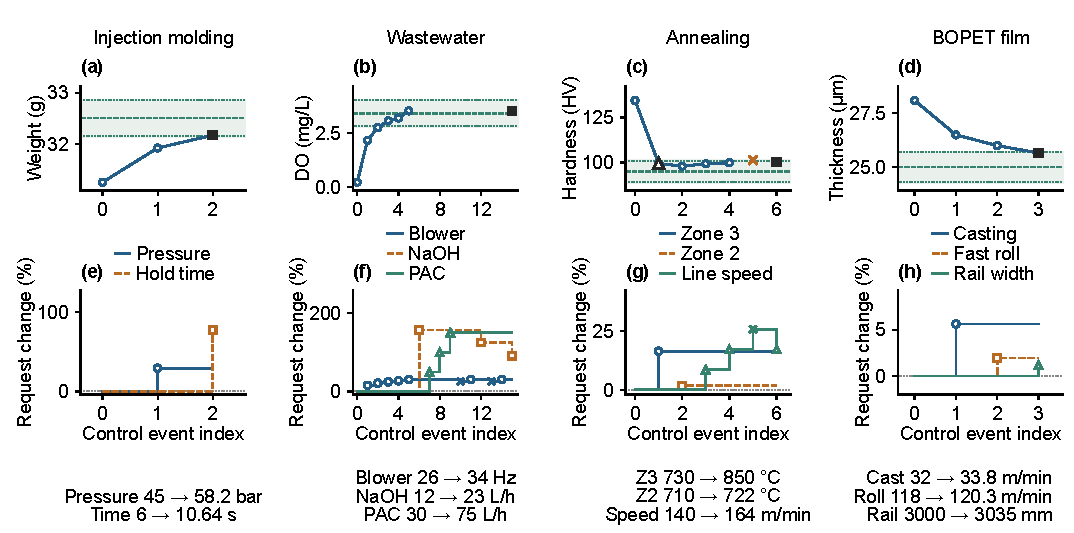
\includegraphics[width=\textwidth]{resources/fig-missions-controls.pdf}
\caption{Historical scripted missions (seed 42, one trajectory per process).
(a--d) Weight, dissolved oxygen (DO), hardness, and film thickness with their
target windows. (e--h) Requested controls as percentage change from native
baselines: injection pressure 45\,bar/time 6\,s; wastewater blower
26\,Hz/NaOH 12\,L/h/PAC 30\,L/h; annealing zone 3
730$^{\circ}$C/zone 2 710$^{\circ}$C/speed 140\,m/min; BOPET casting
32\,m/min/fast roll 118\,m/min/rail 3000\,mm. Lines connect event indices,
not physical time; unchanged requested values carry forward. Crosses mark
reverted candidates and squares distinct terminal observations. The open
triangle in panel (c) marks the first annealing observation, which lacks an
optimization-record ID. DO excludes pH/TP events.}
\label{fig:missions}
\end{figure*}

\subsection{Heterogeneous Protocol Integration and Route Checks (Q1)}
\label{sec:protocol}
The suite acquired \resDaqSamples{} samples over five protocol families and
issued policy-checked writes over four; the RTU-over-TCP line was
acquisition-only.
Archived upper-median write latencies ranged from \resPfiftyRange{}, with observed maxima
\resPninetyfiveRange{}. The four writable lines accepted legal writes and
rejected 24/24 out-of-window probes. A configuration-only second preset
added 9/9 rejected probes on three further writable lines. These results
exercise the same resolver against different signal maps.

In a mock-driver API fixture, three deterministic repetitions of six attack
classes per arm isolated admission from endpoint confirmation. With the
soft-window interlock enabled, both the full and no-readback arms refused
all 18 attacks. Disabling the interlock allowed the six soft-window probes
to execute, while the 12 hard-range probes remained refused. Removing
readback did not change admission, showing that confirmation cannot replace
a pre-write gate. A frozen-measurement drill further separated command and
process evidence: the setpoint and readback agreed, yet the monitoring
quantity remained outside its window and triggered backstop rollback after
\resBackstop{}. A manual-binding drill suspended execution until
harness-issued approval (\resHitlLatency{} mediation span).

\subsection{Live-Engine Tasks and Deterministic Controller (Q2--Q3)}
\label{sec:agentteam}
The archived team workflow linked a parent task, a bound worker, a command,
a verdict, and its journal. On the single-node cast-film mission, the policy
changed the heater from \resMissionFrom{} to
\resMissionTo\,$^{\circ}$C; the observation settled at
\resMissionPv\,$^{\circ}$C within the declared target. The task reached
\texttt{COMPLETED}. The BOPET mission expanded this workflow to nine devices
and 49 signals, with three manipulated nodes
(Section~\ref{sec:scenarios}).

Two live-engine tasks used the same \texttt{omp} harness, Zhipu Coding Plan
provider, and GLM-5.3-Flash model on a scratch line; they are execution
traces, not a strategy comparison or a cross-harness portability test. The archive
records a bounded write, a goal-driven
descent to \resGoalFinal\,$\mu$m for a $52.0\pm0.8$\,$\mu$m target, and a
recipe save. The original contemporaneous omp logs and checked run outcomes
trace proposal, policy-checked action, observations, and retained recipe.
The reported \resGoalFinal\,$\mu$m is the run-summary terminal value;
the log's 52.02\,$\mu$m window mean is a different aggregation.

\label{sec:controller}
A deterministic controller used the dimensionless cast-film objective
\begin{equation}
\begin{aligned}
J={}&55J_{\mathrm{thick}}+25J_{\mathrm{quality}}\\
&+8J_{\mathrm{energy}}+7J_{\mathrm{throughput}},
\end{aligned}
\label{eq:objective}
\end{equation}
whose components score thickness conformance, product quality, and
control-based energy and throughput proxies. The latter two terms use
screw speed and line speed, rather than independently metered energy and
production output. This deterministic-controller experiment is not an
evaluation of AgentWorkShop's optional model service. Table~\ref{tab:q3search}
summarizes its finite candidate grid and selection rule; component formulas
and replay details are provided in \path{REPRODUCIBILITY.md}.

\begin{table*}[!t]
\centering
\caption{Finite-grid search protocol for the deterministic cast-film
controller in Q3. The reference score is restricted to this grid and is not
a global continuous optimum.}
\label{tab:q3search}
\footnotesize
\setlength{\tabcolsep}{4pt}
\begin{tabularx}{\textwidth}{@{}p{2.4cm}Xp{3.0cm}@{}}
\toprule
Search element & Candidate set or rule & Role in the search \\
\midrule
Objective & Eq.~(\ref{eq:objective}); weights 55/25/8/7 for thickness,
quality, energy proxy, and throughput proxy & Rank eligible steady states \\
Eligibility & Melt temperature 195--225~$^{\circ}$C; melt pressure
$\leq 22$~MPa & Discard ineligible states \\
Equal zone setpoint & 195--225~$^{\circ}$C in 2.5~$^{\circ}$C steps & Search variable \\
Screw speed & 50--200~rpm in 5-rpm steps & Search variable \\
Line speed & 20--120~m/min in 2.5-m/min steps & Search variable \\
Die gap & Fixed at 1~mm & Held constant \\
Selection & Evaluate modeled steady state and retain the highest eligible
score; $J^{*}=89.894$ & Finite-grid reference \\
\bottomrule
\end{tabularx}
\end{table*}

Across seeds 42--44, this single controller made two policy-checked writes per
seed, without rejection. It raised $J$ from approximately
\resJzero{} to $J/J^*=\resControllerMin$--\resControllerMax{}, with
$J^*=\resJstar$ from the admissible setpoint grid. This reference
normalization is restricted to the finite search space.
The result links the controller's native objective to admissible commands
and endpoint evidence, exercising a conventional strategy through the
same execution services.

\subsection{Deployment Composition and Confirmation Semantics (Q5)}
\label{sec:hardening}
The deployment suite composed \resLinesLive{} lines, \resChannelsLive{}
channels, \resDaqOnline{} online DAQ nodes, \resWriteNodesLive{} write nodes,
\resRecipesLive{} recipes, and \resBindingsLive{} bindings on one simulator
host. Its injection workflow exercised proposal, pacing, approval, batch
dispatch, and recipe/readback/mirror comparison. The recorded sources agreed
within their tolerances (maximum deviation \resConsistencyErr{}), confirming
setpoint consistency but not process convergence. S4 remained
\texttt{converged=false}; observation-to-verification at 65\,bar took
96.105\,s. S5 applied 40-to-40.5$^{\circ}$C, refused the next write, and
restored 40$^{\circ}$C after a 66.046\,s wait. These are server/harness spans; approval-to-dispatch spans
were \resHitlDispatchMs{}.

Seven injected fault tests checked receipt grading: a mock acceptance needed
reread, a broker outage failed one parameter while its sibling verified, and
a publish-only endpoint remained unverified despite its broker receipt.
Additional checks covered readback promotion and manual-mode confirmation.
MES application receipts were covered by route tests; the deployment run used
MES only for reads. These outcomes characterize the tested fault conditions,
not real-world fault rates.

\subsection{Operational Recipe Workflow Case Study (Q6)}
\label{sec:recipeexperiment}
R6 is one October 18 injection-simulator trajectory, replayed through OPC UA
setpoints and HTTP quality acquisition. Its source commit, seed, and
per-sensor timestamps are unavailable; a live agent diagnosed insufficient
packing, but the intervention and approvals were scripted. From 45\,bar with
6-s hold time, four approved 5-bar \texttt{recipe\_trial}s each waited 65 s
before a DAQ check. The run saved recipe version 2 but did not apply it.
Table~\ref{tab:q6actions} records the sequence.

\begin{table*}[!t]
\centering
\caption{Recorded Q6 injection-recipe actions and post-wait observations
($n=1$ simulator trajectory). Hold time remained 6\,s; each trial used
harness approval, a 65-s wait, and a 1/1 parameter-verification receipt.}
\label{tab:q6actions}
\footnotesize
\setlength{\tabcolsep}{3.5pt}
\begin{tabularx}{\textwidth}{@{}l c c c c X@{}}
\toprule
Stage & Pressure (bar) & Weight (g) & Flash (\%) & Sink (\%) & Recorded action and outcome \\
\midrule
Baseline & 45 & 31.28 & 0 & 1.977 & No command; initial observation \\
Trial 1 & 45$\rightarrow$50 & 31.49 & 0.014 & 1.956 & Approved; 1/1 verified; continue \\
Trial 2 & 50$\rightarrow$55 & 31.74 & 0.031 & 1.760 & Approved; 1/1 verified; continue \\
Trial 3 & 55$\rightarrow$60 & 32.05 & 0 & 1.534 & Weight below 32.15-g minimum and sink above 1.50\%; continue \\
Trial 4 & 60$\rightarrow$65 & 32.30 & 0.019 & 1.277 & Stop recorded; displayed values are within ranges \\
Save & 65 & --- & --- & --- & \texttt{recipe\_update} saved version 2; no \texttt{recipe\_apply} is archived \\
\bottomrule
\end{tabularx}
\end{table*}

R6 disabled per-line trial cadence and bypassed the separate recipe-operation
interval; approval, admission, and command confirmation remained active.
Melt temperature was missing, and the stop used only weight, flash, and sink
mark. The freshness check used the newest available timestamp, so it does not
prove simultaneous per-sensor freshness. We report the recorded stop with
displayed values in range, not an independently audited guard pass; the later
update rationale contains unlinked quality values. A separate 65-to-70\,bar
check began from another state and is not a replicate. In October 23 boundary
checks, the public route refused eight direct-node writes; the default-cadence
recipe route verified one trial, then refused later proposals and failed to
restore the 45-bar baseline (4/8 assertions passed). These are separate
failed boundary records, not repetitions of R6.
